% !TeX spellcheck = en_US

\chapter{Add new package manager module}\label{chap:add}
This chapter shows the extensibility of the framework by adding a new $aptitude$ package manager module for the $bash$ language.\\
Section \ref{sec:aptitude} provides a common information about the $aptitude$.\\
In section \ref{sec:aptitude_imp} the module is implemented and in section \ref{sec:aptitude_int} is integrated into the $bash$ language module.

\section{Aptitude}\label{sec:aptitude}
This section describes the $aptitude$ package manager.
Like to the $apt$-$get$, the $aptitude$ is a command line program, where a package can be installed using the $aptitude$ $install$ \emph{package} command. 
In additional, it can be started in a pseudo-graphical mode to provide a visual interface (An example in figure \ref{fig:aptitude_gui}).
\begin{figure}[ht]   
	\centering
	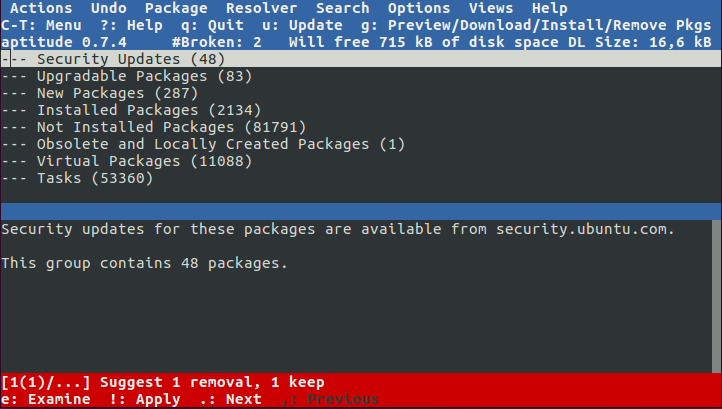
\includegraphics[width=0.7\textwidth]{Screenshot_aptitude.png}
	\caption{A command line visual interface for the $aptitude$ package manager.}
	\label{fig:aptitude_gui}
\end{figure}
An another advantage compared to the $apt$-$get$ is the capability to search for packages by a part of the name (or by any other attributes) using the $aptitude$ $search$ $text$ command.
\section{Implementing the new package manager module}\label{sec:aptitude_imp}
The implementation of the $aptitude$ module will be described here.
At first, the $aptitude$ class will be inherited from the abstract class $PackageManager$. 
This is presented in the listing \ref{lst:aptit_inher}.\\
\begin{Listing} 
\caption{The $aptitude$ inherited from the $PackageManager$ abstract class}
\label{lst:aptit_inher}
\begin{lstlisting}
public final class PM_aptitude extends PackageManager {
	@Override
	public void proceed(String filename, String source)
		throws FileNotFoundException, IOException, JAXBException {
		// TODO Auto-generated method stub
	}
}
\end{lstlisting}
\end{Listing} 
After that, the $aptitude$ class can be used as a regular package manager module (but it lacking functionality).
It is necessary to add the common code, like the constructor and the manager's name.
After these operations, the $ansible$ module can be presented in the listing \ref{lst:aptit_common}.\\
\begin{Listing} 
\caption{The $aptitude$ module with some common elements}
\label{lst:aptit_common}
\begin{lstlisting}
public final class PM_aptitude extends PackageManager {

	// name of the package manager
	static public final String Name = "aptitude";
	
	/**
	* Constructor
	*/
	public PM_aptitude(Language language, CSAR_handler ch) {
		this.language = language;
		this.ch = ch;
	}
	
	@Override
	public void proceed(String filename, String source)
		throws FileNotFoundException, IOException, JAXBException {
		// TODO Auto-generated method stub
	}
}
\end{lstlisting}
\end{Listing} 
Since the package manager will read files from an input CSAR, the CSAR handler is stored by the constructor to the $ch$ variable for a further use.
In addition, the language ($bash$ in this case) is stored too, to be propagated later to the package handler.\\
Now focus on the $proceed$ function.
A line-by-line file analyzer is needed, which can modify the data and in the case of a modification, the entire file should be rewritten.

\begin{Listing} 
\caption{The aptitude $proceed$ function}
\label{lst:aptit_proceed}
\begin{lstlisting}
@Override
public void proceed(String filename, String source)
	throws FileNotFoundException, IOException, JAXBException {
	if (ch == null)
		throw new NullPointerException();
	System.out.println(Name + " proceed " + filename);
	BufferedReader br = new BufferedReader(new FileReader(filename));
	boolean isChanged = false;
	String line = null;
	String newFile = "";
	while ((line = br.readLine()) != null) {
		// TODO parsing will be done here
	}
	br.close();

	if (isChanged)
		Utils.createFile(filename,newFile);
}	 
\end{lstlisting}
\end{Listing} 
The $isChanged$ variable indicates that the file must be rewritten with a new content from the $newFile$ variable.
Now an $aptitude$ line parser will be implemented, which reads a line from the $line$ variable and stores it or it's changed version to the $newFile$ variable.
If the data is changed, then the $isChanged$ variable must be set to true.
Any $ansible$ package installation calls should be detected, commented out and its arguments (package names) should be propagated one by one to the package handler's function $getPackage$.\\
\begin{Listing} 
\caption{The aptitude line parser}
\label{lst:aptit_parse}
\begin{lstlisting}
String[] words = line.replaceAll("[;&]", "").split("\\s+");
// skip spaces at the beginning of string
int i = 0;
if (words[i].equals(""))
	i = 1;
// looking for aptitude 
if (words.length >= 1 + i && words[i].equals("aptitude")) {
	// aptitude found
	if (words.length >= 3 + i && words[1 + i].equals("install")) {
		System.out.println("aptitude found:" + line);
		isChanged = true;
		for (int packet = 2 + i; packet < words.length; packet++) {
			System.out.println("package: " + words[packet]);
			ch.getPackage(language, words[packet], source);
		}
	}
	newFile += "#//References resolver//" + line + '\n';
} 
else
	newFile += line + '\n';
\end{lstlisting}
\end{Listing} 
During the parsing which is described in the listing \ref{lst:aptit_parse}, the line is divided into words. 
Each found package name is transmitted to the packet handler as an argument of its public function $getPackage$.
In additional, this function must take the language and the source artifact's name as the arguments.

\section{Integrating Aptitude into the Bash module}\label{sec:aptitude_int}
Now the $aptitude$ module can be added to the bash module.
The only thing to do is to add the $aptitude$ to the bash's list of package manager modules (the list is stored in the \emph{packetManagers} variable).
This is done by the bash's constructor with the command: \emph{"packetManagers.add(new PM\_aptitude(this, ch));"}.\\
The new package manager module is ready to work.